\documentclass[11pt, a4paper]{article}
\usepackage{graphicx} % Required for inserting images
\usepackage{amsmath}
\usepackage{titlesec}
\usepackage{blindtext}
\usepackage{hyperref} % Para links, en contenido. 
\usepackage{systeme}
\setcounter{section}{-1}

\hypersetup{
    colorlinks=true,
    linkcolor=blue,
    filecolor=magenta,      
    urlcolor=cyan,
    pdftitle={Overleaf Example},
    pdfpagemode=FullScreen,
    }

\renewcommand*\contentsname{ Contenido :} % Para la tabla de contenido

\title{ {\color{blue} Lista de Ejercicios - 1ero BT} }
\author{ Anthony de los Santos \footnote{ Los ejercicios y comentarios presentados aqu\'i son de mi responsabilidad, por cualquier
error visto contactar  \textit{agregdelossantos@gmail.com} } }
\date{ 2024 }

\begin{document}

% ----------- Titulo y contenido

\maketitle 

\newpage

\tableofcontents

\newpage

% ------------


\vspace{20px}

\section{ Sobre estas notas. }

Estas notas estan pensadas para ser una guia en las clases, y tambi\'en ser\'a referencia 
de ejercicios a realizar. 

--- \\
Estas notas, apuntes, estan en construcci\'on. Se modifica en el correr del curso. ~ ~ \textbf{ {\color{red} Ultima modificaci\'on : Lunes 10 de Junio } }

--- \\

\section{ Lista 01: Geometr\'ia }

En esta lista de ejercicios trataremos los temas de Geometr\'ia e introducci\'on a Funciones. De Geometr\'ia veremos mediatriz, bisectriz y sus aplicaciones. Lo ultimo de esta lista ser\'ia el concepto de Funci\'on, esto es, dominio, codominio, representaci\'on de funciones. \\

\subsection*{ Ejercicio 1 }

a) Defina Lugar Geom\'etrico (LG). \\
b) Exprese la Circunferencia como LG. \\
%c) Exprese el algor\'itmo para la construcci\'on de un tri\'angulo equilatero e is\'osceles. 
\subsection*{ Ejercicio 2 - Primeras construcciones }
\subsubsection*{Mediatriz}
En este ejercicios trabajaremos con el concepto de Mediatriz y bisectriz.\\ \\ 
Comencemos con algo simple, dado un segmento de recta $AB$ , de longitud 5cm construir su mediatriz.  \\ 

\textbf{ Ejercicio a) } Construir un tri\'angulo equilatero de lados 6cm y construir la mediatriz en cada uno de sus lados. \\ \\ 
Al construir la mediatriz de cada lado de un tri\'angulo, veremos que se intersectan en un punto, a este punto le diremos \textit{{\color{blue}circuncentro} del tri\'angulo}.\\
Sabemos de Eucl\'ides, que dado un punto (centro) y una distancia (radio) podemos trazar una circunferencia \textit{{\color{blue}(circunferencia circunscrita)}} . Pongamos como centro el punto circuncentro del tri\'angulo y como radio la distancia de este punto a uno de sus vertices. \\ Al construir esta circunferencia, Que podremos notar ? \\

\textbf{ Ejercicio b) } Trace un tri\'angulo escaleno, halle el circuncentro de tal tri\'angulo y trace la circunferencia. \\ \\


\begin{center}
    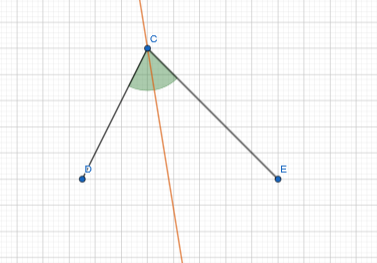
\includegraphics[width = 4cm]{bisectrizDCE.png} 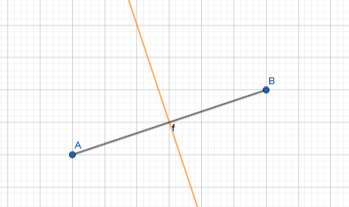
\includegraphics[width = 4cm]{mediatrizAB.png} \\ 
    \small{1) Izquierda: Bisectriz del \'angulo en el vertice C. 2) Derecha: Mediatriz del segmento AB. }
\end{center}


\subsubsection*{Bisectriz}

\textbf{ Ejercicio c) } Construcci\'on de un tri\'angulo is\'osceles con dos lados de 6cm y determinar la bisectriz de cada uno de sus \'angulos. \\ \\ 
Al realizar esta construcci\'on, las rectas se intersectan en un punto, el \textit{{\color{blue}incentro}} del tri\'angulo. Si dejamos como centro de una circunferencia este punto (incentro) y como radio la distancia de tal punto  hacia un lado del tri\'angulo, Que podemos decir de esta circunferencia \textit{ {\color{blue} (circunferencia inscrita) } } ? \\ \\
\textbf{ Ejercicio d) } Construir un tri\'angulo equilatero de lados 7cm. Hallar los puntos circuncentro e incentro de tal tri\'angulo con las respectivas circunferencias. \textit{Trazar cada circunferencias con distinto color, si es posible}

%\subsection{Mediana}
%En un tri\'angulo se denomina {\color{blue}Mediana} al segmento que une un v\'ertice con el punto medio del lado opuesto a dicho v\'ertice. Las medianas se intersectan en un punto llamado {\color{blue}Baricentro} o centro de gravedad. \\ \\
%\textbf{ Ejercicio e) } Encontrar el baricentro de un tri\'angulo equilatero y tambi\'en de un tri\'angulo is\'osceles. 

%\newpage

\subsection*{ Ejercicio 3 - Problemas a resolver }

\subsubsection*{ Pintar la ruta }

En un tramo de ruta nacional, se debe pintar la divisi\'on de carriles sobre una l\'inea que equidista de los lados de la ruta. Supongamos un tramo donde sus lados son rectas paralelas (no hay curvas en este segmento de ruta). Como podr\'ia resolver este problema ? \textit{ a esta l\'inea de pintura la llamamos {\color{blue} paralela media} } \\ \\
Adem\'as de resolver el problema, explicar el m\'etodo usado. 


%\subsection{ Tres punto no alineados }
%\begin{center}
%\includegraphics[scale = 1]{problema3-01.png} \\
%\small{Figura 1) Configuraci\'on de tres puntos en el plano. $A,B,C$}
%\end{center}
%Dado tres puntos en el plano, como en la figura 1), identificar los puntos del plano que equidistan de $A$ y $B$ y estan a 4cm del punto $C$

\newpage

\subsubsection*{ Placa met\'alica }
Para el dise\~no de una pieza met\'alica, se tiene una placa cuadrada de 5cm sus lados. Se necesita  en este dise\~no colocar un disco met\'alico que sea interior a esta placa y que sea tangente a sus lados. Adem\'as se pide un anillo de aluminio de modo que \'este toque los v\'ertices de la placa, de modo que la placa met\'alica estar\'a dentro de tal anillo. \\ 
Construir dicha pieza con las especificaciones indicadas. 

%\newpage

\subsection*{ Ejercicio 4 - Introducci\'on a Funciones }

a) Defina funci\'on entre dos conjuntos A, B. {\color{blue}$( f: A \to B )$}. \textit{(Puede apoyarse de lo visto en clase como en otros materiales (libros, internet,
...) )}  \\ \\
%b) Crear una funci\'on cualquiera, identificando el dominio, codominio y expresando algunos valores de tal funci\'on como ejemplo. \\ \\ \\ 
c) \textbf{ Funci\'on a partir de gr\'afico. } Identificar si corresponde o no a una funci\'on seg\'un el gr\'afico. \\
\begin{center}
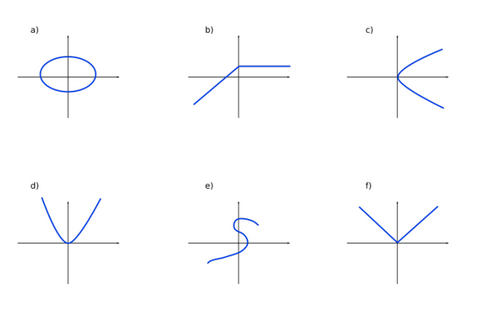
\includegraphics[scale = 0.8]{graficaFuncion.png}
\end{center}
d) Expresar el \'area de un circulo como una funci\'on de su radio. Esto es, dado un radio {\color{blue}(entrada)}, que la funci\'on retorne el \'area del circulo {\color{blue}(salida)}. Crear una \textit{tabla de valores} con la funci\'on con 3 valores como ejemplo. 

\newpage

% Segunda lista 

\section{ Lista 02: Funciones de Primer grado }

En esta lista de ejercicios trataremos el tema de Funci\'on de primer grado y sus aplicaciones y un ejemplo de funci\'on proporcional de tipo $f(x) = 1/x$.   \\

\subsection*{ Ejercicio 1 - Im\'agenes y tabla de valores. }
\subsubsection*{ Ejercicio 1.1) } 
Se consideran las siguientes funciones, \\
a) $ f(x) = 2x + 3 $ ~ ~ b) $\displaystyle  g(x) = 2(x-1) $ ~ ~ c) $\displaystyle p(x) = \frac{-3x}{4} - 2 $ \\ \\
Determinar para cada funci\'on la imagen de $x=2,~x=-3,~ x=0,~x=3$. \\ Construir una tabla de valores, agregando valores a su elecci\'on y realizar la gr\'afica de las funciones. 
\subsubsection*{ Ejercicio 1.2) - Movimiento unidimensional de una p\'articula}
Supongamos el movimiento de una part\'icula que se mueve sobre una recta, esto es, describe un movimiento rectil\'ineo. Cuando \'esta part\'icula esta libre de Fuerzas externas actuando sobre ella, no presenta \textit{aceleraci\'on}. De aqu\'i que la particula tendr\'a \textit{velocidad constante}. Otro caso es cuando la part\'icula presenta una \textit{aceleraci\'on constante}, esto es, $a(t) = a$ siendo $a$ un n\'umero real, constante y $a(t)$ la aceleraci\'on de la particula en un instante de tiempo $t$. Cuando la aceleraci\'on es constante, podemos decir que la velocidad de la p\'articula en un instante $t$ puede expresarse como una funci\'on lineal $f(t) = at + b$ \\ \\ 
Sea $v(t)$ la velocidad de la particula \textit{(unidades en $m/s$)} para un instante $t$ \textit{(segundos)}, Describir en cada caso el valor de la velocidad en el tiempo $t$ y graficar la funci\'on $v(t)$ correspondiente: \\ \\ 
a) $v(t) = 2 $,  Determinar $v(2)$, $v(0)$, $v(5)$ ~ (Opcional : Podrias decir si la aceleraci\'on es nula o con un valor distinto de cero, constante ? )  \\ \\ 
b) $v(t) = 4t + 1$, Determinar $v(0)$, $v(5)$, $v(10)$ \\ \\ 
c) $v(t) = -9.8t + 2$, Determinar $v(0)$, $v(2)$, $v(4)$ \\ \\ 

 
\subsubsection*{ Ejercicio 1.3) Ley de Coulomb y proporcionalidad }
Supongamos dos cargas puntuales, $q_1$, $q_2$ separadas a una distancia $r$ entre las mismas. Hechos emp\'iricos expresan que 1) cargas puntuales ejercen fuerza entre s\'i a traves de la l\'inea recta que las une y la magnitud de esta fuerza es proporcional al producto de la magnitud de las cargas. De repulsi\'on si son ambas del mismo signo, de atracci\'on para signos opuestos. 2) La magnitud de la fuerza es inversamente proporcional al cuadrado de la distancia que existe entre ambas. Esto puede expresarse como: La fuerza entre las cargas $q_1$, $q_2$ en funci\'on de $r$, conocida como la Ley de Coulomb, 
\begin{center}
    $ \displaystyle  \vec{F}(r)_{q_1 - q_2} = k \frac{q_1q_2}{r^2} \vec{e_r} $
\end{center}
Supongamos cargas de 1C (Coulomb), $q_1= q_2 = 1$, y comenzamos a variar la distancia entre estas cargas $r$, determinar F(2), F(20), F(200), F(2000), F(20000). \\ \\
Que podemos decir de la Fuerza $\vec{F}$ cuando \\ la distancia entre las cargas aumenta ? Tomar $ k = 9,0 \times 10^9$ \\ \\ 
Investigar la funci\'on, $\displaystyle f(x) = \frac{1}{x}$ para valores reales positivos. $( x > 0 )$. Ver su gr\'afica e interpretar su comportamiento cuando x toma valores "grandes". Esta funci\'on es un tipo de funci\'on inversamente proporcional \\ \\

\subsection*{Ejercicio 2 - Cortes con los ejes }
\subsubsection*{ Ejercicio 2.1) } Dada las siguientes funciones, hallar los puntos de corte con los ejes. Esto es, determinar la ordenada al origen, \textit{(Corte con el eje vertical $Y$)}, esto se dar\'a cuando $x=0$. Corte con el eje de las abscisas, \textit{(corte con el eje horizontal $X$)}, esto se dar\'a cuando $f(x) = 0$. Realizar gr\'afica.  \\ 
a) $f(x) = 2x + 4 $ ~ ~ b) $g(x) = -3(x - 5) $ ~ ~ c) $\displaystyle h(x) = \frac{x}{7} - 7 $ ~ ~
d) $\displaystyle y(x) = \frac{2x}{3} + \frac{3}{2} $ \\ 

\newpage

\subsubsection*{Ejercicio Opcional: Programac\'on}
Escribir un programa (En el lenguage que deseen, Java, Python,c++,...) que determine los cortes con los ejes. Un ejemplo es definir una funci\'on \\ {\color{blue}cortesPrimerGrado(a,b)}, que toma como entrada dos valores (a,b) de tipo Float, y retorna la salida en pantalla los cortes con los ejes (X,Y). \\ \\ 
Verificar aplicando el programa con las funciones del Ejercicio 2.1)

\subsection*{Ejercicio 3)  }
\subsection*{Ejercicio 3.1)  Una poco de Geometr\'ia }
a) Dada la siguiente figura, determinar el valor de $x$. 
\begin{center}
   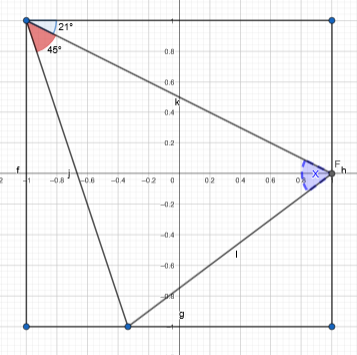
\includegraphics[scale=1]{problemaGeoyFunciones.png}
\end{center}
b) Indicar los cortes con los ejes de la funci\'on, $\displaystyle p(x) = 2x + \frac{\pi}{4}$. \\ \\ c) Resolver $p(x) = \pi$ 

\newpage

\subsubsection*{Ejercicio 3.2) }
Dada las siguientes funciones, $f(x) = 5x - 3$, ~ ~ $\displaystyle g(x) = -\frac{1}{5}x + 3$ \\ \\ 
a) Graficar en un mismo sistema de coordenadas cartesiano, ambas funciones. Esto es, una gr\'afica ambas funciones. Se intersectan estas funciones ? \\ \\
b) Hallar, \textit{si es que se intersectan}, las coordenadas del punto de intersecci\'on. 

% Ejercicio Aplicado. 

\subsection{ Ganancias en la Gomer\'ia }
En un taller de mec\'anica automotriz para el sector de Gomer\'ia deciden incorporar la venta de neum\'aticos. 
Para comenzar con esta propuesta, deciden vender cubiertas rodado 13, R13, de distintas marcas. \\ \\
La administraci\'on obtiene un modelo matem\'atico para estimar la ganancia de ventas, este modelo se expresa como, 
\begin{center}
    $ G(x) = 12 + 40x $
\end{center}
En donde 12 es un valor fijo en Dolares, y por cada neum\'atico vendido, un valor de 40 dolares. \\ \\
a) Convertir cada valor que esta en Dolares a Pesos Uruguayos. \\ \\
b) Calcular la ganancia G(x) si se venden, 5,~8,~10,~13 neum\'aticos. \\ \\
c) Determinar cuantos neum\'aticos se necesitan para que la gancia sea de, \\ \$ 3600, \$ 6880, \$ 11680

\subsection{ Funci\'on Inversa }

\textbf{ a) } Determinar las condiciones para la existencia de una funci\'on inversa de $f: A \to B $ \\ \\
\textbf{ b)  }
Dada las siguientes funciones, hallar la inversa de cada una y realizar una tabla de valores. \\ \\ 
i) $f(x) = 3x - 2$ ~ ii) $ g(x) = 7x + 7 $ ~ iii) $\displaystyle h(x) = \frac{-x}{2} - 3 $ ~ iv) $\displaystyle y(x) = \frac{x}{10}+10$ \\ \\
\textbf{ c) } Graficar 2 funciones de la parte b) con su respectiva inversa. 

 
\end{document}
